%%
% The BIThesis Template for Bachelor Graduation Thesis
%
% 北京理工大学毕业设计(论文)第一章节 —— 使用 XeLaTeX 编译
%
% Copyright 2020-2023 BITNP
%
% This work may be distributed and/or modified under the
% conditions of the LaTeX Project Public License, either version 1.3
% of this license or (at your option) any later version.
% The latest version of this license is in
%   http://www.latex-project.org/lppl.txt
% and version 1.3 or later is part of all distributions of LaTeX
% version 2005/12/01 or later.
%
% This work has the LPPL maintenance status `maintained'.
%
% The Current Maintainer of this work is Feng Kaiyu.
%
% 第三章节
\chapter{系统设计}
{本章将详细介绍系统的各个模块功能及其实现方法。对于在系统实现过程中遇到的挑战与问题,本章会介绍相应算法以及理论方法;对于系统实现过程中各个参数对于系统的影响,本章会进行对比评估。}
\section{系统概述}
{本节主要介绍系统在实现过程中遇到的问题与调整,以及在系统中各个模块的功能和接口。}
\subsection{挑战与问题}
{系统目的是实现利用人体独特的心脏生物特征和移动智能设备上普遍存在的内置摄像头来实现安全有效的用户认证。为了实现这个目标,我们需要解决一下系统设计中存在的挑战与问题。}
\par{首先是需要算法实现可靠的心脏测量。用户心脏生物特征的提取与验证的成功基于对心脏运动模式的可靠测量,又来可靠的心脏运动测量值才能保证系统后续步骤的顺利进行。然而,环境光照条件、指尖按压位置、人体运动情况和心理情绪等因素会影响实际情况下心脏测量结果的可靠性。因此,在系统实现过程中,我们需要一些设备参数调整和噪音过滤算法来获取有效的心脏测量值,缓解这些影响对系统的实现是至关重要的。}
\par
{其次是提取生物独特的心脏特征。用户成功认证离不开有效的心脏特征提取,由于心脏运动模式是通过内置摄像头捕获指尖血流变化间接获得的,因此将记录的视频帧转换为与独特心脏运动模式,并且提取可靠心脏生物特征是一项具有挑战性的任务。此外,为了便于有效的用户认证,从原始心脏测量值中提取具有代表性的生物特征非常重要。当选取的生物特征具有代表性但用于验证又显得数据冗余时,会降低系统进行用户认证的效率,因此需要筛选出代表性强的生物特征,过滤掉一些代表性弱的生物特征,简化系统;当选取的生物特征过于简化,筛选过多时,会使提取的特征无法区分,不具有独特性。因此,筛选并提取具有代表性的生物特征对于系统性能的安全是至关重要的。}
\par
{除此之外,还需提高系统的健壮性。心脏测量还受到许多随机因素的影响,如情 绪变化、心率和呼吸频率的变化。系统应能够消除这种随机性,并得出稳健的生物抽象特征。因此,有必要设计一种能够抑制小尺度心脏运动变化的变换算法来提高系统健壮性。}
\subsection{用户认证模型}
\begin{figure}[htbp]
  \centering
  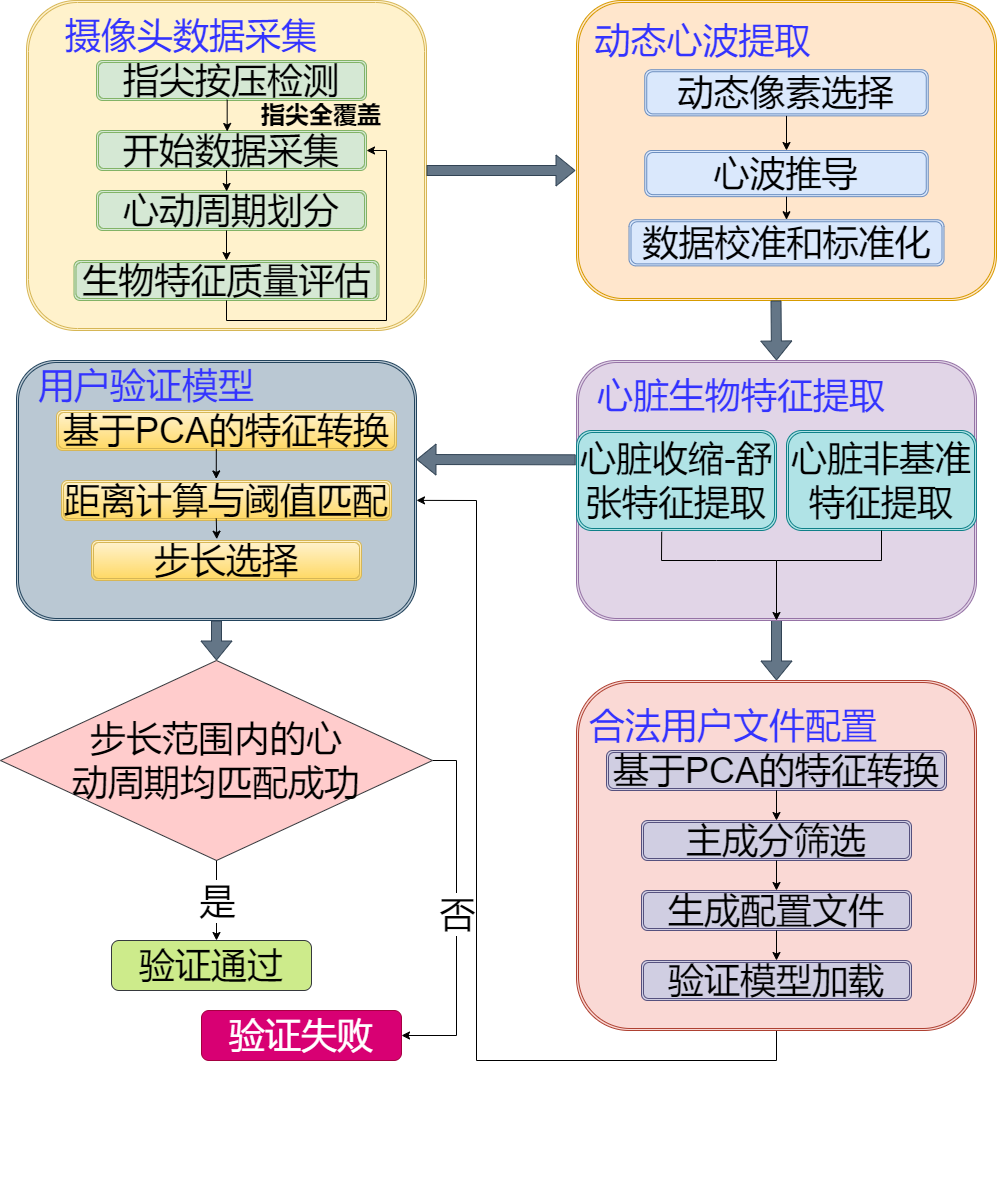
\includegraphics[width=0.53\linewidth]{images/system.drawio.png}
  \caption{系统概述图}\label{3-1} % label 用来在文中索引
\end{figure}
{如图3-1所示,本系统的基本思想是利用普遍使用的移动设备上的内置摄像头和人体独特固有的心脏生物特征来进行用户身份认证。当用户试图访问设备上的隐私信息或使用设备功能时,需要先通过该系统的认证解锁设备释放权限。每次验证一般需要2个心动周期,由于人的心率和使用环境不同,验证时间也有所不同。当用户进行验证时,需要调用算法先检测摄像头获取的图像是否完全被指尖覆盖,当指尖完全覆盖摄像头时验证开始,内置摄像头以视频帧的形式捕捉到指尖的血流,并根据视频帧划分心动周期。在提取特征之前,我们需要对视频帧进行一些优化。由于指尖的按压位置和压力可能在验证过程中保持细微变化,我们通过动态像素选择过滤一些不敏感的像素点,仅处理包括对心脏运动最敏感的像素子集,以提高心脏测量值的信噪比。敏感想读点是在每个心动周期内单独筛选的,通过该心动周期的最大与最小视频帧的差值决定该周期内所有视频帧的掩码进行筛选。然后将所选像素的视频流转换为关于红色、绿色和蓝色通道的三个心波,最后通过带通滤波器过滤掉呼吸和颤抖等人类的生理运动带来的影响。}
\par
{在心脏特征提取模块中,我们直接从处理过的心脏测量值中提取出心脏的收缩-舒张特征,该特征用于描述心脏运动轮廓。在一个心动周期内,从红色、绿色和蓝色通道分别提取10个收缩-舒张特征值。收缩和舒张特征表示为每个心动周期内四个基准点(即舒张点 (DP)、收缩点(SP)、双螺旋切迹(DN)、双螺旋波(DW)\cite{2007Photoplethysmography})之间的标准化距离或斜率。四个基准点用于描述心脏收缩和舒张的四个阶段。可以通过寻找一个心动周期内的局部极大值和极小值(即波峰和波谷)来获取基准点,也可以对基准点位置进行定位。为了提供更多的特征参考,扩大特征空间,我们将原有心波分别通过1Hz和2Hz的高通滤波器获取新的心脏测量值,通过新信号的形态来表现心脏运动的独特性,通过几个基准点的标准化高度差和时间差来描述心脏非基准特征的信号形态。非基准特征在不同用户之间也是唯一独特的。}
\par
{最后,我们通过主成分分析 (PCA)将上述形态特征转化为一组健壮性强的抽象特征。在用户认证时,通过测量用户的心脏抽象特征与配置文件预定义的抽象特征的距离来进行匹配。PCA变换保留了有效区分不同用户的关键特征,同时在选取主分析成分时过滤掉一些特征不明显(归一化方差较小)的特征,简化系统并提升系统性能。如果用户在预定步长的周期内计算的距离均小于预设定的阈值则匹配成功,否则拒绝访问请求。}
%%
% The BIThesis Template for Bachelor Graduation Thesis
%
% 北京理工大学毕业设计(论文)第一章节 —— 使用 XeLaTeX 编译
%
% Copyright 2020-2023 BITNP
%
% This work may be distributed and/or modified under the
% conditions of the LaTeX Project Public License, either version 1.3
% of this license or (at your option) any later version.
% The latest version of this license is in
%   http://www.latex-project.org/lppl.txt
% and version 1.3 or later is part of all distributions of LaTeX
% version 2005/12/01 or later.
%
% This work has the LPPL maintenance status `maintained'.
%
% The Current Maintainer of this work is Feng Kaiyu.
%
% 第四章节

\section{摄像头图像获取与周期划分}
{本节主要讲述摄像头对于手指按压的检测,然后对相机参数调整,以及摄像头图像获取到的图像进行处理,以排除一些环境因素的干扰。}
\subsection{指尖触碰检测}
{
{当手指完全覆盖摄像头时,手指所在区域获取的视频帧的像素点的颜色以红色为主,即血液的颜色。因此当该像素点的红光较强时,可以认为该点被手指覆盖,否则为被手指覆盖,因此可以检查每个像素点的红色通道光强占比,来确定该像素点是否是手指覆盖区域具体公式如下:}
\begin{equation}
    P_{r(x,y)}(t)=\frac{r_{(x,y)}(t)}{r_{(x,y)}(t)+g_{(x,y)}(t)+b_{(x,y)}(t)},(x\in X,y\in Y,t\in T)
\end{equation}
{
其中$r(x,y)$,$g(x,y)$,$b(x,y)$分别表示像素点中红色通道、绿色通道和蓝色通道光强,$X$,$Y$表示帧的宽度和高度,$X\times Y$即摄像头的分辨率,$T$表示所有视频帧。当$P_r(x,y)>\tau$时即认为该像素点被手指覆盖,其中$\tau=0.7$,可根据设备情况与经验进行调整。在当前帧的85$\%$的像素点判定为手指覆盖的红色像素点时,认为该帧被手指完全覆盖,可以开始心波推导。
}
}
\par
{下图分别是手指半遮盖和遮盖时摄像头获取的图像:}
\begin{figure}[htbp]
\centering
    \subfigure[手指半遮蔽]
    {\begin{minipage}[t]{0.2\textwidth}
        \centering
        \renewcommand{\thefigure}{(a)}
        
\includegraphics[width=1\textwidth]{images/halfcover.jpg}
        % \caption{手指半遮蔽}
        \label{3-2}
    \end{minipage}
    }
    \subfigure[手指全遮蔽]
    {\begin{minipage}[t]{0.2\textwidth}
        \centering
        \renewcommand{\thefigure}{(b)}
        
\includegraphics[width=1\textwidth]{images/cover.jpg}
        % \caption{手指全遮蔽}
        \label{3-3}
        \end{minipage}
        }
    \caption{手指覆盖验证}
\end{figure}

\par
{当手指半覆盖时,所有像素点的平均$P_r$值为0.5763,$P_r(x,y)>\tau$的像素点占11.80\%;当手指全覆盖时,所有像素点的平均$P_r$值为0.8893,$P_r(x,y)>\tau$的像素点占100\%。}

\subsection{心跳周期划分}
{心跳周期划分是继续后续实验的基础步骤,后续实验都将单个心跳周期作为数据处理的基本单位进行处理。}
\par
{周期性心脏运动导致指尖血流的规律性变化,在摄像机视频中表现为像素值的各个通道光强变化。为了捕获心脏运动的生物特征,我们需要通过像素值的变化来进行心跳周期的划分,从而进一步提取心脏生物特征。首先需要计算视频流中每一帧的红色通道像素值,以此获取心脏测量值的时间序列。之所以选择红色通道,是因为血液以红色为主,红色通道对血流变化最为敏感。计算平均值公式如下:}
\begin{equation}
    \overline{r}(t)=\frac{\sum_{x,y}{r_{(x,y)}(t)}}{X\times Y}
\end{equation}
\par
{
计算出视频流每一帧的平均红色通道像素值$\overline{r}(t)$后,利用峰谷检测算法\cite{2011Reporting}来获取波谷以切分心动周期。然而一个心动周期内存在多个干扰波谷,为了提升数据的准确性,将某个点的取值扩大到包含这个点的一段区间,用区间内$\overline{r}(t)$的平均值来进行判断,这个区间就是窗口。移动窗口就是窗口向一端滑行,默认是从左往右,每次滑行并不是区间整块的滑行,而是一个单位一个单位的滑行。设置$window$大小为9(可根据经验或实际设备情况进行调整),则从第5帧起,每一帧及其左右各4帧作为一个窗口,窗口内的点的平均值作为划分心动周期的参考值来进行波谷检测,公式如下:
}
\par
\begin{equation}
    r_{rolling}(t)=\frac{\overline{r}(t-\frac{wimdow}{2})+\dots+\overline{r}(t)\dots+ \overline{r}(t+\frac{wimdow}{2})}{window}
\end{equation}
\par
{通过$ r_{rolling}(t)$获取的波形仅用于趋势预测,对于30fps的视频流,一个心波周期以0.8s计算大概为24个视频帧,大小为9的窗口计算出的$ r_{rolling}(t)$的波形存在一定的相位差,因此通过$ r_{rolling}(t)$进行波谷检测后,寻找$\overline{r}(t)$的波形图中最近的波谷,计算$dist=|peak_{r}-peak_{rolling}|$,$dist$值最小的点即作为心动周期的划分点。}
{
对于划分出的心动周期,过滤掉帧数小于最小心动周期的划分(设置最小心脏跳动时间$t_{heart}$,最小帧率为$ t_{heart}\times fps$)。使用上述方法进行心跳周期划分,划分效果如图3-3所示。
}

\begin{figure}[htbp]
  \centering
  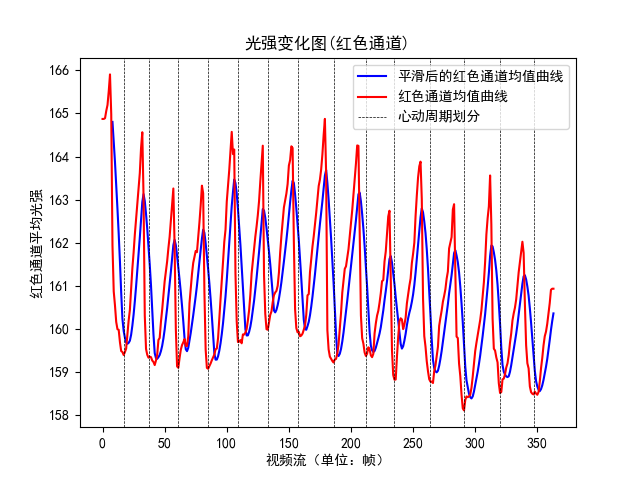
\includegraphics[width=0.9\linewidth]{images/Figure_37.png}
  \caption{心跳周期划分}\label{3-4} % label 用来在文中索引
\end{figure}
\par
{图3-3中红色曲线为采集的视频流中每一帧所有像素点红色通道均值(即$\overline{r}$的曲线),蓝色曲线是将红色曲线在大小为9的窗口上进行平滑操作后得到的曲线。可以看出,蓝色曲线比红色曲线光滑,并且没有突出度较小的波峰波谷,所以使用这条曲线进行波谷查找。图3-3中的黑色虚线代表心动周期划分结果,两条黑色曲线之间之间的帧归属同一个心动周期。}
\par
{上述的心跳周期的分割将适应与之后的心脏特征提取,之后的特征提取将按照单个心跳周期进行处理。}

\par
{心动周期划分结束后,对于每一个心动周期进行处理,通过评估心动周期中的像素值变化(各个通道的光强度变化)来考察像素的灵敏度,并根据灵敏度进行一些合理调整。}
\par
{首先计算每个心动周期的像素逐差$ Diff(r(x,y)) $,其表示一个心动周期中,红色通道像素平均值$ \overline{r} $最大与最小视频帧的差值,公式如下:}

\begin{equation}
    Diff(r(x,y))=r_{(x,y)}(t_{max})- r_{(x,y)}(t_{min})
\end{equation}

\begin{equation}
    Diff(g(x,y))=g_{(x,y)}(t_{max})- g_{(x,y)}(t_{min})
\end{equation}

\begin{equation}
    Diff(b(x,y))=b_{(x,y)}(t_{max})- b_{(x,y)}(t_{min})
\end{equation}
{
其中$t_{max}$和$t_{min}$分别表示表示一个心动周期中,红色通道像素平均值$\overline{r}$最大视频帧与最小视频帧,绿色和蓝色通道的Diff也是同理计算,计算所得的Diff是一个$size=(X,Y,3)$大小的矩阵,与输入的视频帧同样大小。
}
\par
{在计算出$Diff$后,使用k个区间的频率分布直方图来作为评估参数,将0$\sim$255分为k个均等的区间,统计每个区间内$Diff( r )$中像素点落在这个区间内的频率,以此来计算$score$评估参数,公式如下:}
\begin{equation}
    score=\sum_{i}^{k}{i^2\times \frac{|H_i|}{X\times Y}}
\end{equation}
{其中$H_i$表示$Diff( r ) $中落入第$i$个区间的像素点的数量,$score$的值越高表示视频流中红色通道的光强变化越明显,提取特征更容易、更有效,$Diff$和$score$可以用于闪光灯调整和后续图像特征增强作为参考使用。}
\par
{当评估参数$score$过大时,适当调低摄像头闪光灯亮度;当$score$过小时,适当提高摄像头闪光灯亮度。当周围光线较好或摄像头在生物特征提取时对光线要求不高,环境光线对特征提取五影响或影响较小时,也可以不开启摄像头使用。}

%%
% The BIThesis Template for Bachelor Graduation Thesis
%
% 北京理工大学毕业设计(论文)第一章节 —— 使用 XeLaTeX 编译
%
% Copyright 2020-2023 BITNP
%
% This work may be distributed and/or modified under the
% conditions of the LaTeX Project Public License, either version 1.3
% of this license or (at your option) any later version.
% The latest version of this license is in
%   http://www.latex-project.org/lppl.txt
% and version 1.3 or later is part of all distributions of LaTeX
% version 2005/12/01 or later.
%
% This work has the LPPL maintenance status `maintained'.
%
% The Current Maintainer of this work is Feng Kaiyu.
%
% 第五章节

\section{动态心波提取}
{在特征提取过程中,需要排除环境噪音(如周围环境光线变化)和认证过程中人的生理变化(如呼吸、手指按压力度、情绪等)的干扰,以提取出较为可靠的心脏特征。}
\subsection{像素动态选择}
{我们初步探讨发现,不同像素点在相机上感知到的光强度受到多种因素的影响,包括指尖血管分布,手指按压位置,手指按压力度,周围光线变化等。因此,我们需要设计一种合理的策略来过滤一些无效的像素点。首先,我们需要计算一个心动周期中像素点红色通道的平均值,然后获取最大平均值与最小平均值的视频帧,然后计算最大与最小红色像素平均值的视频帧的元素差值,即上一章节计算的$Diff$,然后根据差值的大小获取一个掩码$M$来过滤变化消极的无用像素点,具体公式如下:}
\par
\begin{equation}
M^k(r(x,y))=\left\{
	\begin{aligned}
	1 \quad Diff^k(r(x,y))>\gamma\\
	0 \quad Diff^k(r(x,y))\leq \gamma
	\end{aligned}
	\right
	.
\end{equation}
{其中,$Diff^k(r(x,y))$是第k个心动周期中像素$(x,y)$的红色通道元素差值。基于我们对不同受试者收集的指尖按压数据采集进行的实验效果,根据经验判断取$\gamma =5$,以确保基准特征 (即收缩点和双循环点)可以正确推导,其次还兼顾了用户心跳特征收集后文件配置效果,即不同用户(包括配置文件的用户和攻击用户)采集的测试数据与配置文件的比对效果。当$\gamma$设置过小时测试区分效果不明显,当$\gamma$设置过大时,会将把有效像素点也过滤掉导致测试时攻击用户与原配置的用户的特征提取效果几乎没有没有区别。采集合法用户和非法用户的数个心动周期图像进行效果对比,通过计算提取抽象特征后与合法用户文件配置的抽象特征的距离(Dist(s)的计算会在后续章节介绍)来体现效果,数据如下表:}
% \begin{longtable}{c|c c c|c c c} 
%     \caption{不同$\gamma$值下特征提取效果对比}\label{table5-1} \\
%   \toprule
%    &\multicolumn{3}{c|}{ 合法用户} &\multicolumn{3}{c}{ 非法用户}   \\
%     \hline 
%     $\gamma$ & $dist_{max}$ & $dist_{average}$ & $dist_{min}$  & $dist_{max}$ & $dist_{average}$ & $dist_{min}$ \\
%     \hline
% 0(不进行掩码筛选)& 5.3832 &3.3793 &2.4504 &17.3709 &8.8921 &5.1922  \\ 
% 5& 5.0045 & 3.6607&3.0743 &19.8142 &10.2920 &5.1535 \\ 
% 10&18.9088  &7.9276 &4.6950 &20.8938 &10.8848 &6.2108 \\ 
% 13& 19.4582 &10.7955 &6.9212 &20.2182 &10.2655 &6.7445 \\  \bottomrule
%     \end{longtable}

\begin{table}[htbp]
  \linespread{1.5}
  \zihao{5}
  \centering
  \caption{不同$\gamma$值下特征提取效果对比}\label{table5-1} 
  \begin{tabular}{c|c c c|c c c}
  \toprule
   &\multicolumn{3}{c|}{ 合法用户} &\multicolumn{3}{c}{ 非法用户}   \\
    \hline 
    $\gamma$ & $dist_{max}$ & $dist_{average}$ & $dist_{min}$  & $dist_{max}$ & $dist_{average}$ & $dist_{min}$ \\
    \hline
0(不进行掩码筛选)& 5.3832 &3.3793 &2.4504 &17.3709 &8.8921 &5.1922  \\ 
5& 5.0045 & 3.6607&3.0743 &19.8142 &10.2920 &5.1535 \\ 
10&18.9088  &7.9276 &4.6950 &20.8938 &10.8848 &6.2108 \\ 
13& 19.4582 &10.7955 &6.9212 &20.2182 &10.2655 &6.7445 \\  \bottomrule
    \end{tabular}
\end{table}
\par
{由表3-1可知,当$\gamma=0$(即不进行掩码筛选)时,合法用户和非法用户的抽象特征具有明显的区分度;当$\gamma=5$时,合法用户和非法用户的抽象特征具有明显的区分度,并且非法用户的特征与文件配置的合法用户的特征的距离无论方差还是均值明显增大,合法用户特征虽然与配置文件特征的距离均值略有增大,但是增幅远小于非法用户,并且数据方差减小,$dist$明显收敛,提升了合法用户和非法用户提取的心脏特征的区分度;当$\gamma=10$时,合法用户和非法用户的抽象特征具有的区分度在减小,特征提取效果变差;当$\gamma=13$时,合法用户和非法用户的抽象特征几乎没有区分度。当$\gamma=15$时,某些心动周期的$Diff$值均小于$\gamma$,所有像素点均被过滤。}
\par
{通过上述步骤获取的掩码矩阵具有与视频帧相同的大小,并且应用于一个心动周期中的所有帧。在此后生成配置文件和录入手指按压图像进行用户认证时,应当保证在相同的$\gamma$值下提取特征。}
\subsection{心波推导}
{在上一节中我们获取了所有敏感像素点(即血流引起的光强变化明显的点)的掩码,尽管所有敏感像素都可以捕获血流变化,但是从单个像素点获取心脏特征测量值计算开销大,而且特征复杂冗余。虽然可以额外获取指尖血管分布、指尖皮肤厚度等信息,想要从单个像素点获取心脏特征值提取难度大,用户身份认证也不需要如此多的特征。此外,还应兼顾在不同设备,不同光线环境、用户不同的生理状态和心理状态的情况进行心波推导,使系统在不同的情况下能推导出相似的心波。为了提高系统的健壮性,我们需要简化心波推导过程并保留心脏特征的独特性。因此,我选择使用一个心动周期内的像素点在三个颜色通道(红色、绿色、蓝色)的平均值进行跨模式的心波推导,基于通过掩码筛选出的像素点推导心波,根据以下公式导出单个周期的每一帧的三个通道的心脏测量值:}
\par
\begin{equation}
    W_c^k(t)=\frac{\sum_{x,y}{M^k(x,y)}\times c_{(x,y)}^k(t)}{ \sum_{x,y}{M^k(x,y)}}
\end{equation}
{
其中$ W_c^k(t)$和$ c_{(x,y)}^k(t)$表示第$t$帧在像素点$(x,y)$出的三色通道的光强,是一个$size=(3)$的一维向量(即向量$(b.g.r)$)如等式所示,通过像素矩阵乘以掩模,仅敏感像素值参与心波产生。
}
\par


\subsection{数据校准}
{
根据研究证实,用户本身的呼吸、手指的颤抖、以及一些设备的缺陷也会影响测量本身。
先前的研究发现呼吸对心脏测量的影响通常出现在小于0.3Hz的频段上\cite{Chon2014Respiratory}。为了进一步减轻呼吸、颤抖等与心脏跳动频率不匹配的噪音的干扰,采用通频带为 0.3Hz$\sim$10Hz的$Butterworth$带通滤波器\cite{1975Theory}对心波进一步除杂。
}
\par
{带通滤波实现算法如下:}
\begin{algorithm}
        \caption{带通滤波}
        \begin{algorithmic}[1] %每行显示行号
        \State $fps=30$ \hspace{12em}{\#设置采用频率}
        \Function {bandpass}{} \hspace{8em}\space\space{\#设置阶数为10,带通频率为0.3Hz$\sim$10.0Hz}
            \State $b, a = butter(10, [0.3,10.0], btype='bandpass', fs=fps)$
            \State $red = filtfilt(b, a, W_c(r))$\hspace{3em}\space\space{\#对红绿蓝三个通道分别进行滤波}
            \State $green = filtfilt(b, a, W_c(g))$
            \State $blue = filtfilt(b, a, W_c(b))$
        \EndFunction
        \end{algorithmic}
    \end{algorithm}
\par
{另外,一些于情绪相关人类的生理和心理因素(比如运动、休息和一些心理变化等)都有可能对心跳频率、强度和心跳的规律性有较大的影响,因此心跳幅度和持续时间会有不同的变化。为了让心波推导简化,保证系统在生物特征提取时具有健壮性,我们将把每个心动周期的振幅归一化在$[0,1]$的区间内,以此来减轻或消除心率和心跳强度对特征提取的影响,具体公式如下:

}

\begin{equation}
    y_r(t)=\frac{W_{c(r)}(t)- W_{c(r)}(t_{min})}{ W_{c(r)}(t_{max})- W_{c(r)}(t_{min})}	
\end{equation}
\begin{equation}
    y_g(t)=\frac{W_{c(g)}(t)- W_{c(g)}(t_{min})}{ W_{c(g)}(t_{max})- W_{c(g)}(t_{min})}
\end{equation}
\begin{equation}
    y_b(t)=\frac{W_{c(b)}(t)- W_{c(b)}(t_{min})}{ W_{c(b)}(t_{max})- W_{c(b)}(t_{min})}
\end{equation}
\begin{equation}
    x=\frac{t}{T-1}
\end{equation}
{其中,$ y_r(t)$、$ y_g(t)$、$ y_b(t)$分别代表归一化后三色通道上心跳测量值,即心跳幅度的时间序列,x表示归一化后的横坐标即以一个心跳周期时间为单位标准化后的时间。归一化后,最高振幅为1,最低振幅为0。}
\par
{在获取三色通道通过掩码过滤的平均测量值后,我们分别将三色通道的测量值进行信号处理,过滤掉0.3Hz$\sim$10Hz的信号后得到三色通道的图像如3-4所示:}
\begin{figure}[H]
  \centering
  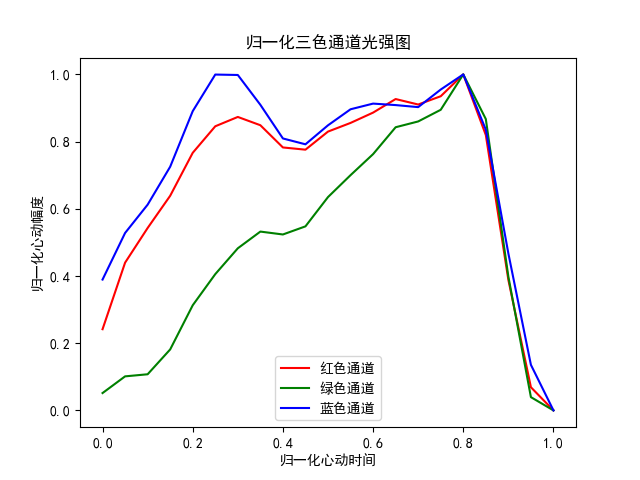
\includegraphics[width=0.65\linewidth]{images/Figure_36.png}
  \caption{归一化后三色通道的心脏测量值}\label{3-5} % label 用来在文中索引
\end{figure}
\par
{由图3-4可知,心脏特征在三色通道上具有相似的轮廓,但在不同通道上表现出的心脏特征不同,在心脏生物特征提取时三个颜色通道的心脏生物特征均需提取。}

%%
% The BIThesis Template for Bachelor Graduation Thesis
%
% 北京理工大学毕业设计(论文)第一章节 —— 使用 XeLaTeX 编译
%
% Copyright 2020-2023 BITNP
%
% This work may be distributed and/or modified under the
% conditions of the LaTeX Project Public License, either version 1.3
% of this license or (at your option) any later version.
% The latest version of this license is in
%   http://www.latex-project.org/lppl.txt
% and version 1.3 or later is part of all distributions of LaTeX
% version 2005/12/01 or later.
%
% This work has the LPPL maintenance status `maintained'.
%
% The Current Maintainer of this work is Feng Kaiyu.
%
% 第六章节
\section{生物特征提取}
{利用心脏原始的收缩-舒张特征来捕获用户心血管系统在视频流中体现的独特的生物特征。简单来说,收缩-舒张特性是通过心动周期在归一化图像上的振幅来体现的,归一化图像上的振幅代表了血液在摄像头采集位置的血流往返信息,振幅上升则代表血液到达,振幅下降则代表血液离开。一个简单的办法是通过提取收缩-舒张的拐点信息来提取心脏运动的收缩-舒张特征,这些特征与独特的生理特征(例如身高、动脉硬度\cite{2002Determination}等)成比例。通过计算拐点的振幅差值、时间差值、以及两点幅度与时间的比例值等方法来收集特征,这种方法方法既简化了系统,使系统在复杂环境下能进行相似的特征提取,增强系统健壮性,又能较为准确的捕捉心脏收缩-舒张特征。除了提取基准特征(心脏收缩-舒张特征)之外,还可以使用非基准特征来捕获从用户心血管系统继承的独特生理特征。}
\subsection{收缩舒张特征提取}
{心波推导完成后,在设计的系统中,我们首先需要从推导出的心波中提取出30个能体现心脏收缩-舒张功能的特征,即心脏的基准特征,来表现心脏的基本收缩-舒张运动。基准特征针对不同个体包含其具有的不同、独特且不易变化的生物特征,并且这些特征在不同的情绪状态(如焦虑、兴奋、紧张、愉悦等)是相对不变且稳定的\cite{2005ECG}。在不同的生理状态(如运动、休息)和不同的环境因素(如环境光强、光源色差、噪音干扰等)下、进行像素选择、归一化和滤波等排除干扰的数据操作后,也能提取出相对独特、稳定的特征。}
\par
{如下图3-5所示,心动周期的四个阶段由三个基准点分开,分别是舒张峰(DP)、重搏切迹(DN)和收缩峰(SP)\cite{2007Photoplethysmography}。我们在一个心动周期范围内,通过搜索心动周期局部范围的波峰与波谷(极大值与极小值)来确定三个基准点的位置。}
\par
\begin{figure}[htbp]
  \centering
  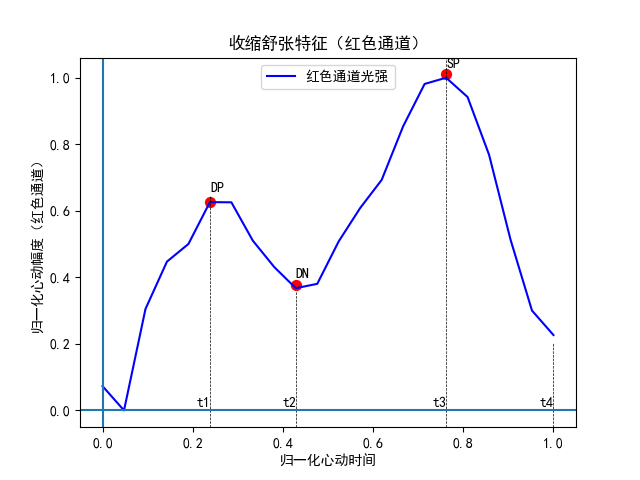
\includegraphics[width=0.8\linewidth]{images/Figure_13.png}
  \caption{收缩舒张特征}\label{6-1} % label 用来在文中索引
\end{figure}
\par
{重博脉指某些病理情况下使正常的重搏波增大,使一次心搏引起的脉波似两次,即收缩期与舒张期各一次,即舒张峰(DP)和收缩峰(SP),常见于肥厚型梗阻性心肌病及长期发热,使外周血管紧张度降低患者。因此舒张峰(DP)、重搏切迹(DN)和收缩峰(SP)也可反应用户的心脏病理特征和血管特征\cite{Evelien2009The}。}
\par
{然而,由于心脏特征具有独特性,并不是所有人的心脏运动都有明显的舒张峰(DP)和重搏切迹(DN)。因此在一个心动周期内,在选定的心波范围内无法找到明显的舒张峰(DP)和重搏切迹(DN)时,由一般心动周期内舒张峰(DP)和双重搏切迹(DN)出现的位置的坐标点作为替代进行特征提取。}
\par
{具体来说,在标准化测量值(即进行归一化和0.3Hz$\sim$10.0Hz滤波后的三色通道光强)和标准化时间间隔内,$t1$、$t2$、$t3$和$t4$分别表示心室射血、等容舒张、心房收缩和等容收缩的持续时间,而标准化振幅值$h1$和$h2$表示相应心脏时相的血流量。在提取$h1$时,选取[0.1,0.3]局部范围内的波峰进行查找,缺省波峰时使用$t=0.2$的值进行替代;在提取$h2$时,选取[0.21,0.45]局部范围内的波谷进行查找,缺省波谷时使用$t=0.35$的值进行替代;在提取$h3$时,选取[0.6,1.0]局部范围内的波峰进行查找,缺省波峰时使用$t=0.8$的值进行替代(一般$h3=1$而且不会缺失)。特别注意$h3$一般是最大振幅值,而$h4$是标准化时间$t=1.0$时的标准化振幅值,即最后一帧的标准化振幅值。此外,还可以用归一化后的斜率$s1$、$s2$、$s3$和$s4$来描述血流变化梯度,具体计算方法为:$s_j=\frac{|h_j|}{t_j},j=1,2,3,4$。由此得到$h_1$、$h_2$、$t_1$、$t_2$、$t_3$、$t_4$、$s_1$、$s_2$、$s_3$、$s_4$一共10个特征值,从每个颜色通道(即红、绿、蓝)三色通道各提取10个特征值,一共30个特征值。}


\subsection{非基准特征提取}
{数据校准过程(即通过截止频率为0.3$\sim$10Hz的带通滤波器)消除了人体呼吸和高频噪音的影响,但是人指尖的略微移动和手握手机时的颤抖也会对心波的生物特征进行干扰,而这些干扰大多大于0.3Hz,并且扭曲包含在心波中的生物特征。因此,我们希望利用高通滤波器来减少指尖运动和颤抖所造成的干扰,进而提取不同的非基准特征。与基准特征相比,非基准特征能更好地表 征每个心动周期的整体信号形态(如形状)。最近的研究\cite{2017Non}表明,可以成功地从PPG信号中获得非基准特征并用以区分用户。}
\par
{具体来说,将原有的心波(红、绿、蓝三个颜色通道)分别通过两个截止频率为1Hz和2Hz的$Butterworth$高通滤波器\cite{1975Theory},分别获得两个非基准心波$w1$和$w2$。}
\par
{具体实现算法如下:}
\begin{algorithm}
        \caption{高通滤波}
        \begin{algorithmic}[1] %每行显示行号
        \State $fps=30$ \hspace{12em}{\#设置采用频率}
        \Function {highpass}{$fre$}\hspace{6em}\space\space{\#设置阶数为10,高通截止频率为$fre$}
            \State $b, a = butter(10, fre, btype='highpass', fs=fps)$
            \State $red = filtfilt(b, a, W_c(r))$\hspace{3em}\space\space{\#对红绿蓝三个通道分别进行滤波}
            \State $green = filtfilt(b, a, W_c(g))$
            \State $blue = filtfilt(b, a, W_c(b))$
        \EndFunction
        \end{algorithmic}
    \end{algorithm}
\par
{图3-6为经过截止频率为1Hz和2Hz的$Butterworth$高通滤波器后得到的单个心动周期的非基准特征图,由几个特征点表征非基准特征的大致表现。}
\begin{figure}[htp]
\centering
    \subfigure[通过1Hz的高通滤波器后提取的非基准特征]
    {\begin{minipage}[t]{0.49\textwidth}
        \centering
        \renewcommand{\thefigure}{(a)}
        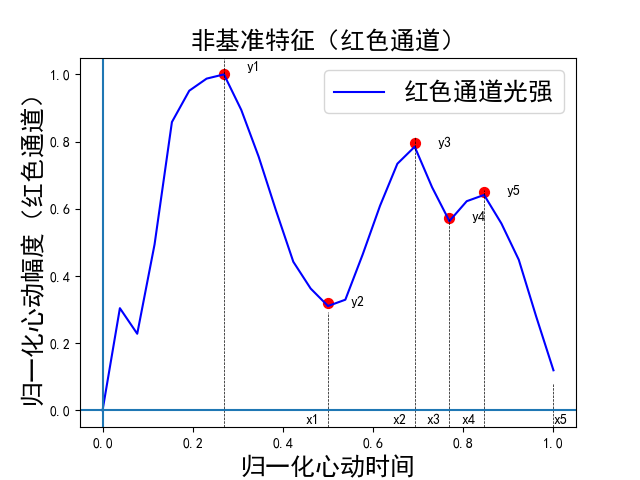
\includegraphics[width=1\textwidth]{images/Figure_34.png}
        \label{6-2}
    \end{minipage}
    }
    \subfigure[通过2Hz的高通滤波器后提取的非基准特征]
    {\begin{minipage}[t]{0.49\textwidth}
        \centering
        \renewcommand{\thefigure}{(b)}
        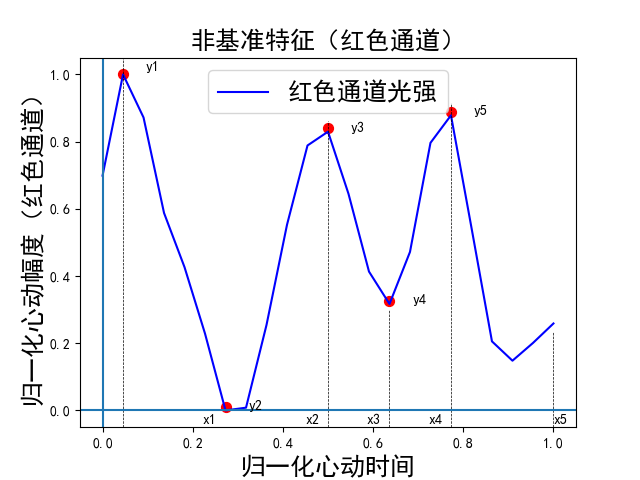
\includegraphics[width=1\textwidth]{images/Figure_35.png}
        \label{6-3}
        \end{minipage}
        }
    \caption{非基准特征}
\end{figure}
\par
{如图3-6所示,$y1,y2,\dots,y5$为归一化后特征点的高度,$x1,x2,\dots,x4$分别表示$y1,y2,\dots,y5$之间归一化后的时间差,$x5$表示$y5$与最后一帧之间归一化后的时间差。}
\par
{$w1$和$w2$的局部波峰和波谷(极大值和极小值)之间的归一化距离对于每个个体都是唯一、独特的,并且一起用作表征心脏运动的非基准特征。因此,我们从两个非基准心波的每个颜色通道中提取6个特征${x1,x3,x5,| y1−y2 |,| y3−y4 |,| y5 |}$。通过查找不同用户之间最显著的水平和垂直峰谷距离来选择这6个特征。同理,由于每个人心脏的独特运动和一些采样过程中的特例导致并非每个人的非基准特征都能在局部归一化范围内找到波峰和波谷,因此一个心动周期内,在选定的心波范围内无法找到明显非基准特征时采用一些定值点的值来替代。在提取$y1$时,选取[0.1,0.3]局部范围内的波峰进行查找,缺省波峰时使用$t=0.2$的值进行替代;在提取$y2$时,选取[0.21,0.45]局部范围内的波谷进行查找,缺省波谷时使用$t=0.3$的值进行替代;在提取$y3$时,选取[0.31,0.6]局部范围内的波峰进行查找,缺省波峰时使用$t=0.5$的值进行替代; 在提取$y4$时,选取[0.5,0.8]局部范围内的波谷进行查找,缺省波谷时使用$t=0.7$的值进行替代;在提取$y5$时,选取[0.7,1.0]局部范围内的波峰进行查找,缺省波峰时使用$t=0.9$的值进行替代。具体的参数更具采样的结果和实验效果而定。}
%%
% The BIThesis Template for Bachelor Graduation Thesis
%
% 北京理工大学毕业设计(论文)第一章节 —— 使用 XeLaTeX 编译
%
% Copyright 2020-2023 BITNP
%
% This work may be distributed and/or modified under the
% conditions of the LaTeX Project Public License, either version 1.3
% of this license or (at your option) any later version.
% The latest version of this license is in
%   http://www.latex-project.org/lppl.txt
% and version 1.3 or later is part of all distributions of LaTeX
% version 2005/12/01 or later.
%
% This work has the LPPL maintenance status `maintained'.
%
% The Current Maintainer of this work is Feng Kaiyu.
%
% 第七章节

\section{用户认证模型}
{随着人的一系列生理活动和情绪变化,心波每天可能会有小规模的变化,因此,我们需要将上述提取的66个特征进行一种特征转换来抑制变化,并基于这种特征转换实现用户心脏特征的匹配。}
\subsection{基于PCA的转换}
{我们需要一种特征转换方案,来构建可靠的用户配置文件,让用户基于PCA\cite{1986Principal}转换进行用户身份认证。具体方法是通过主成分分析(PCA)将原有的高维心脏特征转化为低维空间中的一组正交主成分,并选取其中最具有代表性的前几个主成分(即归一化后方差占比最大的前几个主成分),因为他们特征表现强,对干扰信号具有较强的健壮性(抗干扰性)。}
\par
{具体来说,我们选择用户的70个心波进行特征提取,一个心动周期提取出66个心脏特征值,由此心动周期的特征由70个66维的列向量$a_1,a_2,a_3,\dots,a_{69},a_{70}$组成一个$66\times 70$的矩阵$A_{66\times 70}$表示。同一个向量在不同的基下的表示是不一样的,要准确描述向量,首先要确定一组基,然后计算向量在各个基上的投影值,就能够得到该组基下的向量表示。因此PCA变换的目标是将$A_{66\times 70}$做为原始数据矩阵映射到新的基下并进行降维,矩阵$A_{66\times 70}$拥有70条样本和66个特征(维度),矩阵$U_{k\times 66}$ 为由k个n维向量表示的新空间(一组基),则经过基变换后得到的数据矩阵为:}
\begin{equation}
    F_{k\times 70}= U_{k\times 66}\times A_{66\times 70}
\end{equation}
{其中$F_{k\times 70}$为降维后得到的矩阵,经过基变换后得到的矩阵$F_{k\times 70}$中的70个样本由66维降到了k维。}
\par
{基变换的实质:使用一组基来确定新的维度空间,将原始数据投影到该组基确定的各个维度空间。优化目标需要确定一组合适的基,使得投影后的投影值尽可能分散(不相关)。将原矩阵相似对角化是一种普遍采用的变换法方,然而只有满秩的方阵才能求解特征值和特征向量进行相似对角化,$66\times 70$的矩阵无法进行相似对角化。因此将奇异值分解(SVD)\cite{1993Singular}应用于生物特征矩阵。SVD分解将任意矩阵分解成一个正交矩阵和一个对角矩阵以及另一个正交矩阵的乘积。对角矩阵的对角元称为矩阵的奇异值,可以证明,奇异值总是大于等于0的。当对角矩阵的奇异值按从大到小排列时,SVD分解是唯一的。将矩阵$ A_{66\times 70}$进行如下分解:
}
\begin{equation}
    A_{66\times 70}=U_{66\times 66} \times S_{66\times 70} \times V_{70\times 70}
\end{equation}
{其中$ U_{66\times 66}$ 和 $V_{70\times 70}$分别是矩阵$AA^\intercal$和矩阵$A^\intercal A$特征值和特征向量求解后得到的正交基,$S_{66\times 70}$是分解得到的奇异值矩阵,奇异值按由大到小对角排列。对66个心脏特征进行PCA转换时只需对$A_{66\times 70}$的列向量进行降维,因此只需使用奇异值分解(SVD)得到的矩阵$ U_{66\times 66}$作为PCA转换的基,导出主分析成分。算法实现如Algorithm 4所示。}
\begin{algorithm}[!ht]
        \caption{PCA转换}
        \begin{algorithmic}[1] %每行显示行号
        \State load  70  cycles \hspace{8em}\space\space\space {\#获取70个合法用户心跳周期}
        \State $\tau =0.9$
        \State $Features$ is empty
        \For  {cycle in cycles}
            \State $feature$ is empty
            \State bandpass() \hspace{8em} \space \space{\#消除呼吸和高频噪音影响并提取基准特征}
            \State $feature$.append(cycle.getSystolicDiastolicFeature())
            \State highpass(1) \hspace{8em} {\#消除1Hz以下的干扰频率影响并提取非基准特征}
            \State $feature$.append(cycle.getNonfiducialFeature(1Hz))
            \State highpass(2) \hspace{8em} {\#消除2Hz以下的干扰频率影响并提取非基准特征}
            \State $feature$.append(cycle.getNonfiducialFeature(2Hz))
            \State $Features$.append($feature$)
        \EndFor
        \State $A_{66\times 70}=Features^{T}$
        \State $U_{66\times 66} \times S_{66\times 70} \times V_{70\times 70}=A$ \space {\#将矩阵$A$进行奇异值分解}
        \State $W_{66\times 70}=U_{66\times 66}\times A_{66\times 70}$
        \State sort $w_1,w_2,\dots,w_{66}$ in $W$ by $S^2(w)$ \space {\#将主分析成分按方差 $S^2(w)$从大到小排序}
        \State $sum=0$
        \For {$w$ in $W$}
        \State $sum=sum+\frac{S^2(w)}{\sum_{i=1}^{66}{S^2(w_i)}}$
        \If{$sum\leq\tau$} \hspace{6em} {\#$sum\leq\tau$时保留主成分$w$}
        \State keep $w$ 
        \Else \hspace{11em} \space\space {\#$sum>\tau$时舍弃主成分$w$}
        \State drop $w$ 
        \EndIf
        \EndFor
        \end{algorithmic}
    \end{algorithm}
\newpage
\par
{
由70个心动周期观测值的心脏特征组成,得到主成分$W={w1,w2,\dots ,w70}$,其中$wj,j=1,\dots ,66$表示n维主成分向量。首先,我们需要计算这70个向量每一个向量的方差,并且将这些向量按照方差由大到小进行排列。接下来,我们选择前k个标准化方差最大主成分,称为心脏具有最大标准化方差的抽象特征。由于所有的心动周期都具有相似的前几个主成分,这些主成分描述了导出的心波的形态轮廓,其余的主成分能够更好地区分不同的个体。因此,我们丢弃前两个主成分,并从第三个主成分开始主成分选择过程。主成分选择过程满足以下目标函数:
}
\begin{equation}
    k=max\left\{ k|\sum_{j=3}^{k}{\frac{S^2(w_j)}{\sum_{i=1}^{66}{S^2(w_i)}}}<\tau,k<66\right\}
\end{equation}
{其中k是所选主分量的数量,$\tau=0.9$是预定义的阈值,该阈值是根据经验确定的,以平衡性能与计算复杂度之间的权衡。当$\tau$过大时会保留大多影响较小特征而影响计算性能,当$\tau$过小时会过滤掉一些影响较大的有用特征,用户识别时匹配效果不好。$\tau=0.9$过滤了大多数影响小的心脏抽象特征,简化了系统。}
\par
{通过摄像头提取了志愿者的70个心动周期的图像用于生成系统的合法用户配置文件,共采集2757帧,摄像头帧率(fps)设置为30,一共划分出105个心动周期(只取前70个用于生成配置文件),心率为67次/分钟。将由70个心动周期获取心脏特征由66维降到40维,过滤掉约40\% 的影响较小的心脏抽象特征}
\par
{将选出的主分析成分和主分析向量生成文件进行保存,用于后续验证时的配置文件匹配。具体来说,需要用于降维的一组基(即矩阵$ U_{66\times 66}$)进行保存,后续匹配时的特征转换也需要这组基将特征进行映射,同时还应记录选出的k组主分析成分的索引,在使用矩阵$ U_{66\times 66}$进行PCA转换后选出对应索引的主分析成分,以保证匹配时转换后的心脏抽象特征与配置的合法用户的心脏抽象特征对应。除此之外,还应记录经过PCA转换后得到的70组k维的抽象特征,用于距离匹配。}
\subsection{配置文件匹配}
{在选取70个心跳周期进行PCA特征转换后,我们将形成的特征保存成为配置文件。在进行用户心脏特征匹配时,我们通过测量新捕获的心脏抽象特征(即经过PCA转换后的特征)与已形成主分析成分的心脏抽象特征(70个k维向量)之间的相似度来进行用户认证。一般来说,从向量的角度看,来自合法用户的心脏抽象特征应该与合法用户本人的个人资料(即生成的用户心脏抽象特征配置文件)有较小的距离,而没有得到授权的非法用户捕获的心脏抽象特征应该与配置的抽象特征距离较远。}
\par
{
我们使用一组心脏抽象特征$F={f1,f2,\dots ,f70}$进行匹配,这组向量源于合法用户配置 文件中的70个心脏周期提取的特征进行PCA转换后得到的抽象特征。对于每个心动周期
将提取的心脏特征向量($66\times 1$维)经过一组基组成的矩阵$ U_{66\times 66}$映射后得到心脏抽象特征。具体来说将矩阵$ U_{66\times 66}$与特征向量($66\times 1$维)相乘后得到在新的特征空间$ U_{66\times 66}$下的心脏抽象特征,然后通过配置文件保存的k组主成分索引选出对应的主成分完成降维。根据上一节中描述,每个新捕获的请求验证的心波都将进行基于PCA的特征变换,以获得心脏抽象特征$s$。然后, 我们计算每个$s$和$F$之间的平均欧氏距离(即二范数),如下所示:
}
\begin{equation}
    Dist(s)=\frac{\sum_{i=1}^{n}{|f_i-s|}}{n}
\end{equation}
{其中,$f_i$是配置文件中的第$i$个心脏抽象特征,我们使用阈值$\eta$来进行特征匹配:如果$Dist(s)\leq \eta$,则用户认证成功;否则验证失败,表明检测到攻击者或未经授权的用户尝试获取手机权限。}

\par
{为了获得优化的阈值$\eta$,我们的系统既需要合法样本,也需要一些模拟欺骗攻击的非法用户样本来检测和评估预定义的阈值。我们可以利用约登指数的J统计量来对阈值进行评估\cite{2014Shoulder},计算公式如下:}
\begin{equation}
    J=sensitivity+specificity-1
\end{equation}
\par 
{对参数进行如下解释:}
\par
\begin{itemize}
    \item {\textbf{灵敏度(sensitivity):}}{又称敏感度,是指筛检方法能将实际有病的人正确地判定为患者的比例,在本实验中为合法用户心波匹配成功的概率;}
    \item {\textbf{特异度(specificity):}}{是指筛检方法能将实际无病的人正确地判定为非患者的比例,在本实验中为攻击用户心波验证失败的概率;}
\end{itemize}
\par
{$J(\eta)$是一个单一的统计量,用于表现识别攻击者和合法用户的性能,并选择具有最大J统计量的阈值。具体来说就是满足以下函数:$\eta=argmax(J(\eta)),\eta \in S$,其中$S$为提供阈值选择的所有样本距离集合。}
\par
{当获取最优阈值$\eta$后,我们同样得到阈值$\eta$对应的灵敏度(sensitivity)和特异度(specificity),计算得到的阈值$\eta$是在对每个心动周期进行认证的情况下得到了。处于安全情况考虑考虑,为了提高系统的健壮性,我们在验证时选取$n$个周期进行验证,当$n$个周期内的心动周期都低于阈值$\eta$时认为验证通过,因此此时在非法用户进行验证时成功拒绝的概率和在合法用户认证通过的概率分别如下:}
\begin{equation}
    sensitivity(n)= sensitivity(1)^n
\end{equation}
\begin{equation}
    specificity(n)=1-(1.0- specificity(1))^n
\end{equation}
\begin{equation}
    J(n)= sensitivity(n)+ specificity(n)-1
\end{equation}
{其中$sensitivity(n)$表示取$n$个周期进行认证,当$n$个周期都通过认证(即$n$个周期内均满足$dist \leq \eta$的情况下)的灵敏度(sensitivity),$sensitivity(1)$即上述求最优$\eta$时得到的$sensitivity$;$ specificity (n)$表示取$n$个周期进行认证,当$n$个周期中存在认证不通过(即$n$个周期内存在$dist>\eta$的情况下)的特异度(specificity),$ specificity (1)$即上述求最优$\eta$时得到的$ specificity $。当$J(n)$最大时取得的$n$值作为认证时选取的用户心跳周期数,计算$J(n)$使用实际数据测试得到的概率而不用理论计算得到的概率。但是为了系统安全性考虑,攻击用户认证拒绝的成功概率需要由较高值是用户隐私才能具有安全性,在损失少量系统性能(即提高$n$值,损失部分$sensitivity(n)$,从而延长验证时间)的情况下,适当提高系统安全性。验证时选择的周期数可以根据实验数据与结果进行综合考虑决定。}